Una onda es una perturbación o fluctuación que se propaga a través de algún medio transportando energía. Se caracteriza por la porpagación de una perturbación a través de un medio.

La palabra `onda' deriva de la palabra en latín `unda', que significa ola, oleada o agua agitada.

Las ondas transfieren energía, no materia. En ciertas ocasiones, esa energía se puede interpretar como información significativa.

\begin{grafica}
\centering
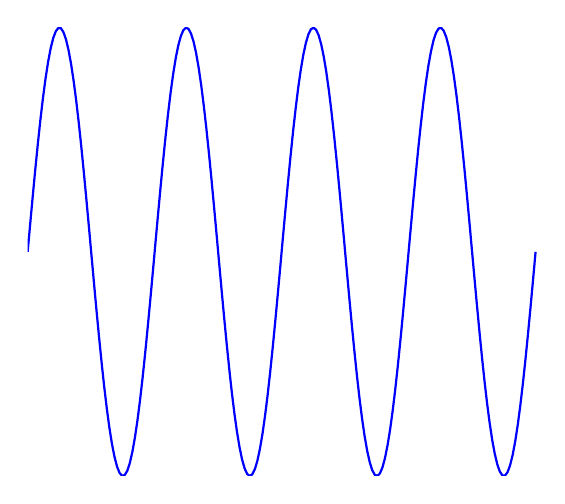
\begin{tikzpicture}
  \begin{axis}[
    xmin=0,xmax=8.5*pi,
    ymin=-1,ymax=1,
    axis lines = none,
    xtick={0},ytick={0}
    ]
    \addplot[color=blue,samples=200,domain=0:8*pi,thick]{sin(deg(x))};
  \end{axis}
\end{tikzpicture}
\caption{Onda simple}
\end{grafica}
